% !TeX root = main.tex
%% Chapter02-激光及激光雷达系统.tex
%% 激光及激光雷达系统
\chapter{激光及激光雷达系统}

\section{激光} %% Section 1 	激光
\textit{激光}(Light Amplification by Stimulated Emission of Radiation, Laser),即“光的手机辐射放大”。

\subsection{辐射与原子} %% Subsection 1.1	辐射与原子
\paragraph{辐射与原子的相互作用的三种过程} \begin{enumerate}
	\item 
		\textit{自发辐射跃迁}:较高能级的粒子,自发地发射一个光子,跃迁到较低能级。其过程如图\ref{fig:自发辐射跃迁}所示。
		\begin{figure}[htbp]
			\centering
			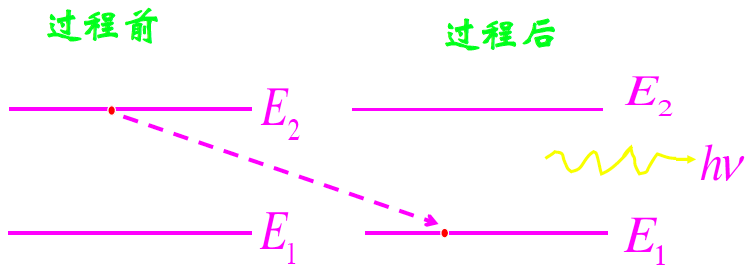
\includegraphics[width=0.7\linewidth]{figure/Chapter2/自发辐射跃迁}
			\caption{自发辐射跃迁}
			\label{fig:自发辐射跃迁}
		\end{figure}
		
		\textbf{光子的频率}为\begin{equation} \nu = \dfrac{E_2-E_1}{h} \end{equation}其中,$ h $是普朗克常量,$ h=6.624 \times 10^{-34} \ \symrm{\mu m} $。
		
		\textbf{自发辐射的速率}为\begin{equation} A_{21} = \dfrac{\diff n_{21}}{\diff t} \dfrac{1}{n_2} \end{equation}
		自发辐射速率的倒数表示由自发辐射所决定的有限寿命\begin{equation} \tau = \dfrac{1}{A_{21}} \end{equation}
		
		具有两个能级的原子系统在外来辐射的作用下可能产生两种过程:\begin{itemize}
			\item 处于低能级E1的原子在外来辐射作用下,吸收一个光子后向高能级E2跃迁(受激吸收过程);
			\item 处于高能级E2的原子在外来辐射作用下,发射一个与入射光子属于同一光子态的光子,并向低能E1级跃迁(受激辐射过程);
		\end{itemize} % 具有两个能级的原子系统在外来辐射的作用下可能产生两种过程
	\item 
		\textit{受激吸收跃迁}:较低能级的粒子吸收一个光子,跃迁到较高能级。其过程如图\ref{fig:受激吸收跃迁}所示。
		\begin{figure}[htbp]
			\centering
			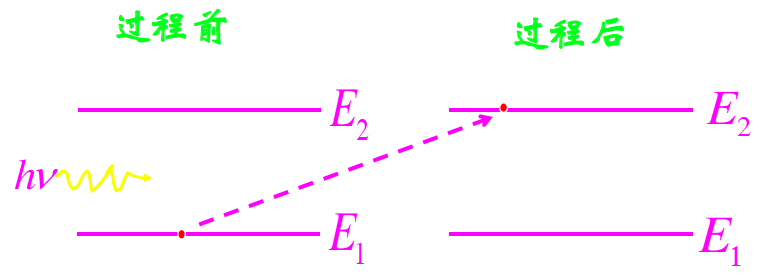
\includegraphics[width=0.7\linewidth]{figure/Chapter2/受激吸收跃迁}
			\caption{受激吸收跃迁}
			\label{fig:受激吸收跃迁}
		\end{figure}
	\item 
		\textit{受激辐射跃迁}:较高能级的粒子在光子激励下跃到较低能级,并发射一个同频率光子。其过程如图\ref{fig:受激辐射跃迁}所示。
		\begin{figure}[htbp]
			\centering
			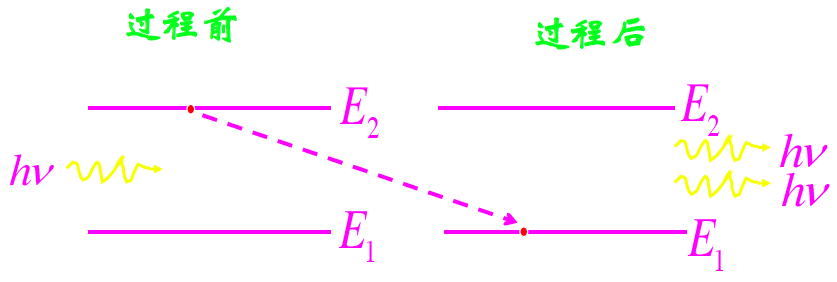
\includegraphics[width=0.7\linewidth]{figure/Chapter2/受激辐射跃迁}
			\caption{受激辐射跃迁}
			\label{fig:受激辐射跃迁}
		\end{figure}
\end{enumerate} % 辐射与原子的相互作用的三种过程

\subsection{受激辐射放大} %% Subsection 1.2	受激辐射放大
\paragraph{外来辐射场的作用}原子系统会产生受激吸收过程和受激辐射过程。\begin{itemize}
	\item \textit{受激吸收过程}:具有一定频率的光子消失的过程,表现为能量由外来辐射场向原子转移,导致辐射场的衰减。
	\item \textit{受激辐射过程}:是原子系统不断产生具有一定频率的光子,表现为能量由原子向辐射场的转移,使辐射场增强。
\end{itemize} % 外来辐射场的作用
一般说来,这两种过程总是同时存在。\begin{itemize}
	\item 如果受激吸收过程占主导地位,最终结果则是辐射场衰减;
	\item 而如果受激辐射过程起主导作用,最终结果就是辐射场的增强。
\end{itemize}% 两种作用同时存在

\paragraph{辐射场增强的条件}在某一段时间$ \diff t $内,由于受激辐射而从能级$ E_1 $向能级$ E_2 $跃迁的原子数为
\begin{equation} \diff n_{12}=n_1W \diff t \end{equation}
由于受激辐射作用而从从能级$ E_2 $向能级$ E_1 $跃迁的原子数为\begin{equation} \diff n_{21}=n_2W \diff t \end{equation}这里假定$ W_{12} = W_{21} = W $。

在两种过程共同作用下,光子的净增量可以表示为
\begin{equation} \Delta N = \left(n_2W - n_1W\right)\diff t = \delta nW\diff t \end{equation}
其中$ \Delta n = n_2-n_1 $。

\textbf{入射光经过原子系统后得到增强的条件}:处于能级E2上的粒子数多于能级E1上粒子数。

根据玻尔兹曼分布定律,处于热平衡状态时,有
\begin{equation} \dfrac{n_2}{n_1} = e^{\frac{E_2-E_1}{kT}} < 1 \end{equation}
即,辐射光通过处于热平衡状态的原子系统时,是辐射场的衰减。

\textbf{粒子反转分布状态}:要使得辐射场得到增强,必须使原子系统的分布为$ n_2>n_1 $。
以某种方式向原子系统提供能量,将足够多的粒子从能级$ E_1 $抽运到$ E_2 $。

\subsection{激光的产生} %% Subsection 1.3	激光的产生
\paragraph{工作物质}原子系统在获得能量后,处于粒子数反转分布状态,称之为\textit{激光工作物质}。工作物质的特点:\begin{itemize}
	\item 工作物质自身某些原子的自发辐射产生的光子, 在传播过程中会作为入射光引起其它原子受激跃迁。
	\item 工作物质处于粒子数反转分布状态,若受激辐射跃迁超过受激吸收跃迁,则光在传播中会得到激励和放大。
	\item 只要工作物质足够长,即使初始信号很小,也会被放大得很强。
\end{itemize}

\paragraph{激光产生的条件}\begin{itemize}
	\item 工作物质处于粒子数反转分布状态。
	\item 受激辐射跃迁超过受激吸收跃迁。
	\item 传播中的光得到激励和放大。
\end{itemize}

\paragraph{激光产生的过程}在工作物质两端分别放置一块反射镜,构成一个\textit{光学谐振腔}。工作物质由抽运系统被抽运到粒子数反转分布状态,因自发辐射而产生的向各个方向传播的光子,在光学谐振腔的作用下,沿着腔轴方向传播的光就会因两端的反射镜往返传播,并很快得到放大。那些传播方向与腔轴方向有一定夹角的光在几次往返后会逸出腔外。由于受激辐射占主导地位,沿腔轴往返传播的光由于受激辐射迅速放大,形成\textit{自激振荡},产生了激光。

受激辐射场与激励场具有相同的频率、相位、传播方向和偏振态,即\textbf{受激辐射光子和激励光子属于同一光子态},所以激光束具有很好的方向性、单色性、相干性。

\begin{figure}[!htbp]
	\centering
	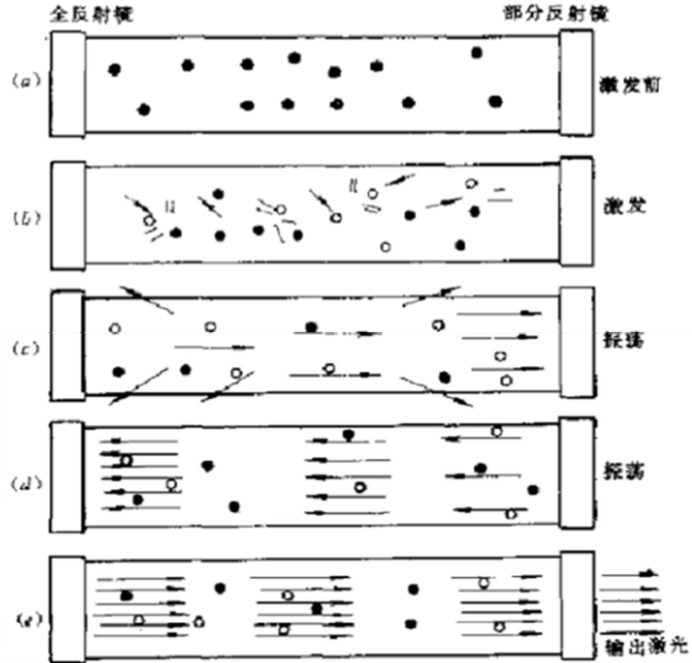
\includegraphics[width=0.6\linewidth]{figure/Chapter2/激光的产生过程}
	\caption{激光产生过程}
	\label{fig:Chpater2-激光产生过程}
\end{figure}

\section{激光器} %% Section 2	激光器

\paragraph{激光器}产生激光的装置称为激光器,激光器虽然多种多样,但其目的都是通过激励和受激辐射放大而获得激光。
\paragraph{激光器的组成}\begin{itemize}
	\item 工作物质
	\item 抽运系统
	\item 光学谐振腔
\end{itemize}
\paragraph{激光器的分类}
\begin{multicols}{2}
	\begin{itemize}
		\item \textbf{按照工作物质分类} 
			\begin{itemize}
				\item 固体激光器
				\item 气体激光器
				\item 液体激光器
				\item 半导体激光器
				\item 自由电子激光器
			\end{itemize} % 按照工作物质分类
		\item \textbf{按转运方式分类}
			\begin{itemize}
				\item 连续激光器
				\item 单次脉冲激光器
				\item 重复脉冲激光器
				\item 锁模激光器
				\item 单模和稳频激光器
				\item 可调谐激光器
			\end{itemize} % 按转运方式分类
		\item \textbf{按激励方式分类}
			\begin{itemize}
				\item 光泵式激光器
				\item 电激励式激光器
				\item 化学激光器
				\item 核泵浦激光器
			\end{itemize} % 按激励方式分类
		\item \textbf{按照输出波段范围分类}
			\begin{itemize}
				\item 远红外激光器
				\item 中红外激光器
				\item 近红外激光器
				\item 可见激光器
				\item 近紫外激光器
				\item 真空紫外激光器
				\item X射线激光器
			\end{itemize} % 按照输出波段范围分类
	\end{itemize}
\end{multicols}

\paragraph{激光的应用}\begin{itemize}
	\item \textbf{自然科学}
	\item \textbf{加工领域}
	\item \textbf{信息处理}
	\item \textbf{激光通信}
	\item \textbf{医学领域}
	\item \textbf{军事领域}
\end{itemize}

\paragraph{未来激光器的发展}
\begin{itemize}
	\item 实用角度
	\item 波长角度
	\item 输出功率
	\item 新类型激光器
\end{itemize}

\subsection{气体激光器} %% Subsection 2.1	气体激光器
\paragraph{用于激光雷达的气体激光器}主要有:\begin{itemize}
	\item \ce{CO2}激光器
	\item \ce{BrHg}激光器
	\item \ce{N2}分子激光器
	\item 准分子激光器
\end{itemize}

工作波长从近紫外到红外;以强放电激励为基本能源。

\paragraph{\ce{CO2}激光器}\ce{CO2}激光器是最早用于激光雷达的激光器之一,工作波长工作波长为10.6 μm,处于大气窗口。至今仍广泛用于激光雷达。

\paragraph{\ce{CO2}分子的震动方式}\ce{CO2}分子的3个原子呈对称排列,震动方式如图\ref{fig:CO2分子的震动方式}所示。
\begin{figure}[htbp]
	\centering
	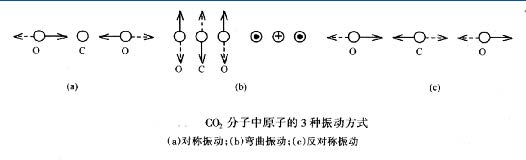
\includegraphics[width=\linewidth]{figure/Chapter2/CO2分子的震动方式}
	\caption{\ce{CO2}分子的震动方式}
	\label{fig:CO2分子的震动方式}
\end{figure}

\paragraph{\ce{CO2}激光器的优点}\begin{itemize}
	\item \ce{CO2}激光器工作波长工作波长为10.6 μm,对人眼安全。
	\item 具有优良的大气传输性能。
	\item 有较大的输出功率和能量转换效率。
	\item 易于进行外差探测。
\end{itemize}

\paragraph{\ce{CO2}激光器的缺点}\begin{itemize}
	\item 需要低温制冷。
	\item 目标对10.6 μm的激光反射率低,且\ce{CO2}激光易被水分子吸收。
\end{itemize}

\paragraph{\ce{CO2}激光器的跃迁机理}
\begin{enumerate}
	\item 
		\textbf{由分子在基态电子能级的振动子能级间跃迁产生}。在放电激励情况下,两种跃迁方式:
		\begin{itemize}
			\item 基态电子能级中(000)振动子能级上的分子与激励电子碰撞,被直接激发到激光能级(001)上,即:
				\begin{equation} \ce{CO2(000) + e\text{(高能)} -> CO2(001) + e\text{(低能)} } \end{equation}
			\item 具有较高的振动子能级分子与其它处于(000)能级上的分子发生碰撞, 跃迁到激光能级(001)。
		\end{itemize}
		两种可能的跃迁方式概率都不大。
	\item 
		\textbf{为了提高跃迁概率,在\ce{CO2}中掺入少量的\ce{N2}气体}。基态电子能级中V=0的振动子能级上的N2分子,被激励电子碰撞后跃迁到V=1的振动能级与CO2的(001)能级接近,很容易将能量转移到处于(000)能级的CO2分子,使它跃迁到(001)能级。即
		\begin{equation} \ce{ CO2(000) + N2(V=1) -> CO2(001) + N2(V=0) } \end{equation}\\
		\textbf{优点}:\ce{N2}分子基态电子能级的V=1子能级寿命相当长,可以积累大量\ce{N2}分子,使较多\ce{CO2}分子从(000)能级跃迁到(001)能级。\\
		\textbf{增加输出功率}:\begin{itemize}
			\item 进一步加入氦气可以使激光输出功率几倍地增大。
			\item 加进适量氙气(\ce{Xe}),也能使其增加输出功率。
			\item 加入适量的水蒸汽(\ce{H2O}),可使激光输出功率显著地增加。
		\end{itemize}
		\textbf{延长激光器的寿命}:在\ce{CO2}激光器里加入氢气(\ce{H2})、一氧化碳(\ce{CO})和氧气(\ce{O2})将延长激光器的寿命。
\end{enumerate}

\subsection{固体激光器} %% Subsection 2.2	固体激光器

\paragraph{常见的固体激光器} Nd:YAG激光器、钛宝石激光器等。

\paragraph{固体激光器的特点}\begin{itemize}
	\item 一般体积较小,与气体激光器相比更加可靠。
	\item 应用十分广泛。
\end{itemize}

\paragraph{Nd:YAG激光器} \begin{itemize}
	\item \textbf{化学组成}:是以钇铝石榴石晶体(化学式是\ce{Y3Al5O15},简称为YAG)为基质,掺入约1\%的激活离子\ce{Nd^3+}就成为Nd:YAG。
	\item \textbf{应用}:用于遥感的Nd:YAG激光器,在典型情况下脉宽10$ \sim $30 ns,单脉冲能量为100 mJ$ \sim $1 J,脉冲重复率为10$ \sim $100 Hz。
		\begin{itemize}
			\item 波长1.06 μm的基频辐射YAG激光器可用于研究大气散射。
			\item 波长0.532 μm的2倍频频光可用于海洋勘探。
			\item 波长0.355 μm和0.266 μm的3倍频和4倍频光可用于测污。
		\end{itemize}
\end{itemize}

\paragraph{二极管泵浦YAG激光器}由于固体激光器在相干性、脉冲重频和输出功率等方面受到局限,遇到CO2 激光器的挑战。寻求新的泵浦方法即二极管泵浦YAG激光器。
\begin{itemize}
	\item \textbf{优点}:泵浦效率高,输出功率高,寿命长。
	\item \textbf{缺点}:结构复杂,成本较高。
\end{itemize}
二极管泵浦Nd:YAG激光器的结构,如图\ref{fig:激光二极管泵浦YAG激光器}所示。
\begin{figure}[htbp]
	\centering
	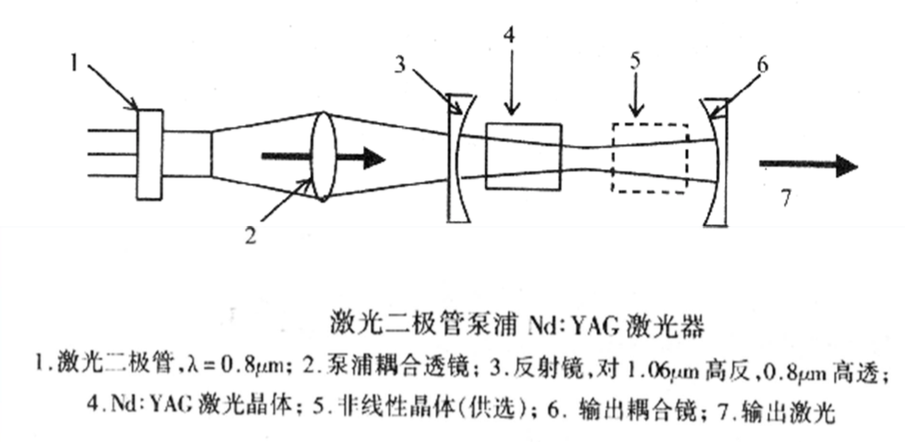
\includegraphics[width=0.7\linewidth]{figure/Chapter2/激光二极管泵浦YAG激光器}
	\caption{二极管泵浦Nd:YAG激光器的结构}
	\label{fig:激光二极管泵浦YAG激光器}
\end{figure}

\paragraph{固体可调谐激光器} 
\begin{itemize}
	\item \textbf{作用}:激光雷达探测对象的响应特性与激光波长密切相关,波长可调的激光器十分有用。
	\item \textbf{类型}:
		\begin{itemize}
			\item 1979年Walling等发明\textit{翠绿宝石激光器}
				\begin{itemize}
					\item 早期有较高实用价值的固体可调谐激光器。
					\item 波长调谐范围是700 $ \sim $ 830 nm。
				\end{itemize} % 翠绿宝石激光器
			\item 1982年Moulton发明\textit{钛宝石激光器}
				\begin{itemize}
					\item 一个重要的进展。
					\item 钛宝石激光晶体的基质是\ce{Al2O3},其中少量的\ce{Al^3+}被\ce{Ti^3+}取代(便于产生激光)。
					\item 钛宝石在400$ \sim $600 nm范围内具有很宽的吸收带,发射带为660$ \sim $1160 nm,波长调谐范围很宽。
					\item 虽然钛宝石具有较大的受激发射截面,增益较高,但激光能级的寿命只有3.2 μs,通常用其它激光器作抽运工作:氩离子激光器、铜蒸气激光器、2倍频Nd:YAG激光器。
				\end{itemize}
		\end{itemize} % 类型
\end{itemize} % 固体可调谐激光器

\subsection{半导体二极管激光器} %% Subsection 2.3	半导体二极管激光器
\paragraph{半导体二极管激光器的特点}
\begin{itemize}
	\item 完全不同的物理机制。
	\item 半导体材料中的电子智能存在于两个能带之一,每个能带所包含的能级数等于晶体中的原子数。根据Pauli不相容原理,每个能级上只能有一个电子。
	\item 半导体材料多是晶体结构。当大量原子规则而紧密地结合成晶体时,晶体中那些价电子都处在晶体能带\footnote{价电子所处的能带称\textit{价带}(对应较低能量)。与价带最近的高能带称\textit{导带},能带之间的空域称为\textit{禁带}}上。本征半导体的能带结构如图\ref{fig:本征半导体能带结构}所示。
		\begin{figure}[htbp]
			\centering
			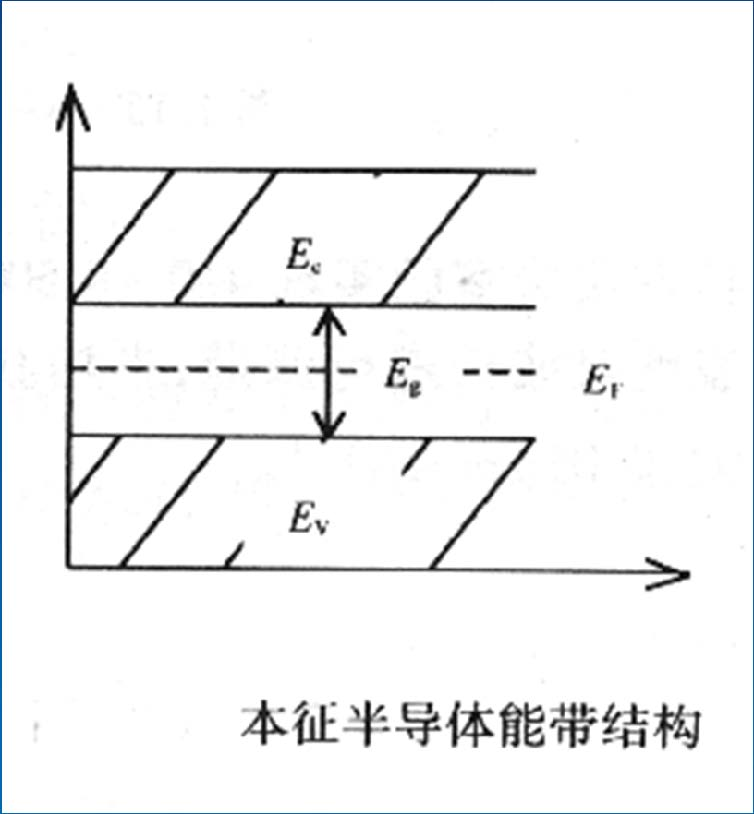
\includegraphics[width=0.3\linewidth]{figure/Chapter2/本征半导体能带结构}
			\caption{本征半导体能带结构}
			\label{fig:本征半导体能带结构}
		\end{figure}
	\item 电子不能再两个能带之间(禁带)驻留。
	\item 没有杂质的纯净半导体,称为本征半导体。
\end{itemize}

\paragraph{半导体二极管激光器的工作原理}
\begin{enumerate}
	\item 如果在本征半导体中掺入杂质原子,则在导带之下和价带之上形成了杂质能级,分别称为施主能级和受主能级。
		有施主能级的半导体称为\textit{n-型半导体};有受主能级的半导体称为\textit{p-型半导体}。
	\item 由于p-半导体与n-半导体所处能级不一致,高低能级的载流子作扩散运动,最终形成\textit{p-n结},此时处于热平衡状态,具有统一的Fermi能级。该过程如图\ref{fig:p-n结}所示。
		\begin{figure}[htbp]
			\centering
			\includegraphics[width=0.5\linewidth]{figure/Chapter2/P-N结}
			\caption{p-n结}
			\label{fig:p-n结}
		\end{figure}
	\item 若加偏压,在结区形成窄区域,导带(高能级)底部能级被电子占据, 价带(低能级)顶部被空穴占据;当导带电子回到价带, 与空穴发生受激复合时就产生了激光。该过程如图\ref{fig:p-n结产生激光}所示。
		\begin{figure}[htbp]
			\centering
			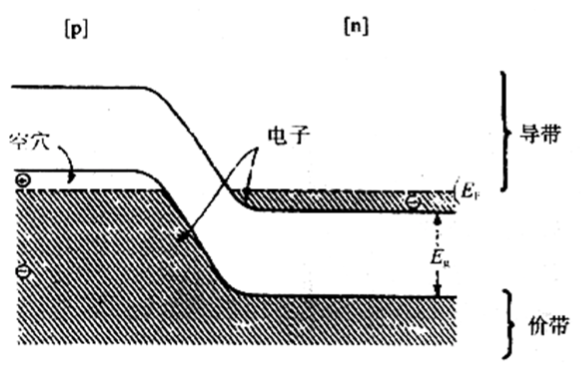
\includegraphics[width=0.5\linewidth]{figure/Chapter2/p-n结产生激光}
			\caption{p-n结产生激光}
			\label{fig:p-n结产生激光}
		\end{figure}
\end{enumerate}

\section{激光雷达系统} % Section 3	激光雷达系统
\subsection{激光雷达系统概述} % SubSection 3.1	激光雷达系统概述

\paragraph{激光雷达的产生}雷达工程师努力探索更短波长的辐射源,在微波振荡器的基础上,发明了激光器,将其与雷达技术相结合,产生了激光雷达技术。

\paragraph{激光雷达的特点}
\begin{itemize}
	\item 角分辨率较高
	\item 距离和速度分辨率高
	\item 抗干扰能力强
	\item 能够与一些目标发生生化作用
	\item 可以对极小的目标进行探测激
\end{itemize}

\paragraph{激光雷达的要求} 激光雷达要求具备发射高功率、窄脉宽、窄频带、较小远场发散角光束较高的脉冲频率的激光器。

\paragraph{激光雷达系统的分类}
\begin{enumerate}
	\item \textbf{按照使用目的分类}
		\begin{itemize}
			\item 探测环境状态
				\begin{itemize}
					\item \textbf{大气}:气溶胶分布、云、气象因素、污染物质……
					\item \textbf{水体}:浮游生物、水温、海洋污染……
					\item \textbf{陆地}:植物生长、热岛效应、污染状况……
				\end{itemize} % 探测环境状态
			\item 量测距离
				\begin{itemize}
					\item \textbf{太空}:星球间距离、星球地形……
					\item \textbf{海洋}:水体深度、水下地形……
					\item \textbf{陆地}:地形图、数字高程模型、植被提取……
				\end{itemize} % 量测距离
		\end{itemize} % 按照使用目的分类
	\item \textbf{按激光和物质的相互作用分类}
		\begin{itemize}
			\item \textbf{反射}:检测比激光波长大很多的物体。地形测绘。
			\item \textbf{米氏散射}:检测微粒直径与激光波长相等的物质。气溶胶。
			\item \textbf{瑞利散射}:检测微粒直径与激光波长小很多的物质。空气分子。
			\item \textbf{拉曼散射}:具有震动和旋转能力的分子。空气分子、水蒸气、\ce{SO2}等污染物质。
			\item \textbf{荧光法}:具有共振能级的分子和原子。\ce{NO2}等污染物质。
		\end{itemize} % 按激光和物质的相互作用分类
	\item \textbf{按使用的激光器分类}
	\item \textbf{按脉冲方式或连续波方式分类}
	\item \textbf{按光波检测的方法分类}
	\item \textbf{按工作台分类}
	\item \textbf{按接收的信号\footnote{激光雷达接收的信号:\begin{itemize}
			\item 可能是反射信号
			\item 也可能是大气散射信号(被称为弹性散射)
			\item 吸收衰减信号、共振散射信号、荧光信号等
	\end{itemize}}分类}
		\begin{itemize}
			\item \textit{反射型激光雷达系统}:地形测绘。
			\item \textit{散射型激光雷达系统}:探测大气中低浓度的尘埃
			\item \textit{吸收性激光雷达系统}:估计某种成分的平均密度
			\item \textit{激光荧光系统}:探测大气中的微量元素
		\end{itemize}
\end{enumerate} % 激光雷达系统的分类

\paragraph{双视场米氏散射激光雷达}武汉大学研制的双视场米氏散射激光雷达,主要由激光发射系统、光学接收系统和信号检测系统组成。

\paragraph{激光雷达系统的结构} 
\begin{itemize}
	\item \textit{双稳系统}:发射部分和接收部分分开放置,目的是为了提高空间分辨率。由于目前脉宽为ns级的激光已达到很高空间分辨率,因此该系统已经很少被采用。双稳系统结构框图如图所示。
		\begin{figure}[htbp]
			\centering
			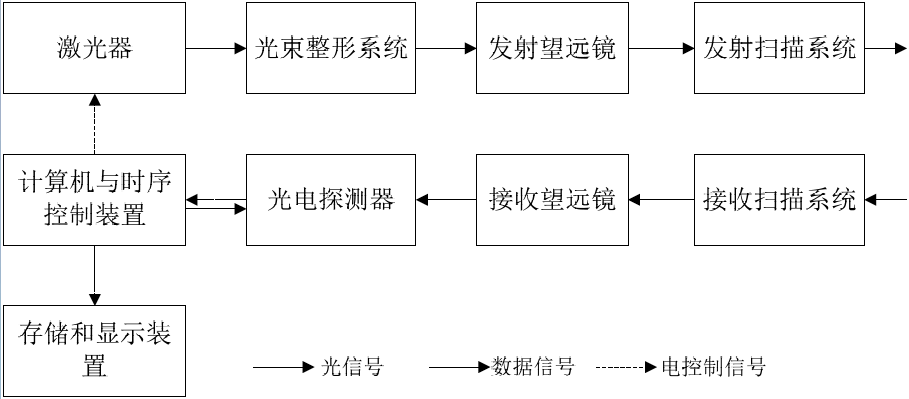
\includegraphics[width=0.7\linewidth]{figure/Chapter2/双稳系统的结构框图}
			\caption{双稳系统的结构框图}
			\label{fig:双稳系统的结构框图}
		\end{figure}
	\item \textit{单稳系统}:发射与接收信号共用一光学子系统,由发送/接收(T/R)开关隔开。单稳系统结构框图如图所示。
		\begin{figure}[htbp]
			\centering
			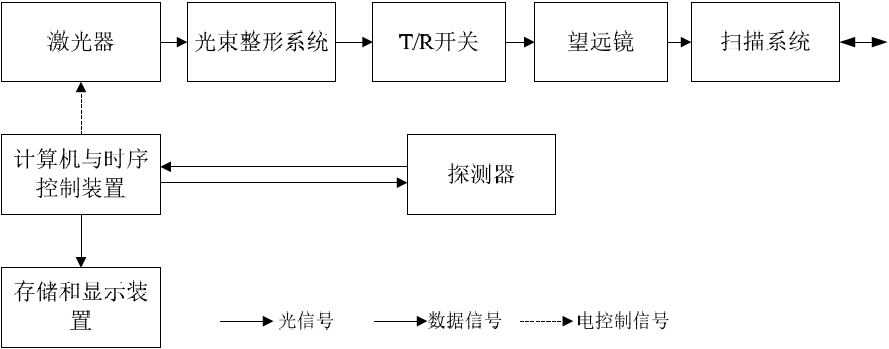
\includegraphics[width=0.7\linewidth]{figure/Chapter2/单稳系统的结构框图}
			\caption{单稳系统的结构框图}
			\label{fig:单稳系统的结构框图}
		\end{figure}
\end{itemize}

\subsection{光束整形} % Subsection 3.2	光束整形

\paragraph{光束整形}通过整形器控制出射激光的指向、方位信息、光束排布状况、束宽等参数,使其形成一定的排布规律,便于检测与分析。

激光器中的光学谐振腔无论是什么形状,其电磁场均具有一定的振荡频率和一定的空间分布,被称为\textit{腔的模式},用$ \mathrm{TEM}_{mn} $表示。其中,$ m = n = 0 $的模称为\textit{基模}。基模场振幅均满足高斯分布,这时激光光束称为\textit{基模高斯光束}。很多情况下要求将基模高斯光束整形为柱状对称,具有平顶强度分布的光束。如图\ref{fig:光束整形}所示。
\begin{figure}[htbp]
	\centering
	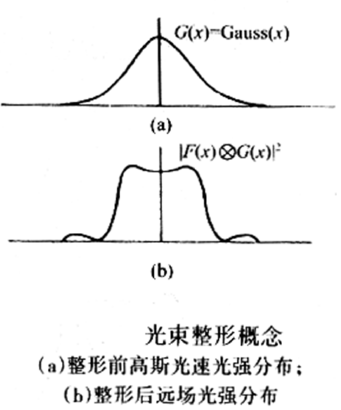
\includegraphics[width=0.3\linewidth]{figure/Chapter2/光束整形}
	\caption{光束整形}
	\label{fig:光束整形}
\end{figure}

\paragraph{光束整形的方法}\textit{衍射光栅}是光束整形的方法之一。光束整形器的能量色散元件由透明二元衍射光栅构成。选择合适的光栅周期和刻线相位调制深度,就可以达到所要求的整形效果。

\subsection{激光扫描} % Subsection 3.3	激光扫描

\paragraph{激光扫描}在光束整形之后,采用某种技术使激光束发生偏转,实现对某区域的目标进行扫描。

\paragraph{激光扫描技术的分类}
\begin{itemize}
	\item \textbf{高惯性扫描}
		\begin{itemize}
			\item 机械技术或反射镜棱镜技术
			\item 主要靠反射镜或棱镜的旋转实现扫描
		\end{itemize} % 高惯性扫描
	\item \textbf{低惯性扫描}
		\begin{itemize}
			\item 电光棱镜的梯度扫描
			\item 振动反射镜的非梯度扫描
			\item 增益控制或损耗控制的内腔式扫描
		\end{itemize}
\end{itemize} % 激光扫描技术的分类

\paragraph{衍射光学元件(DOE)}可替代旋转平面反射镜或棱镜,省去了机械转动部件,减少了折射元件数量,能对任意非球面误差进行校正。如图\ref{fig:衍射光学元件}所示。
\begin{figure}
	\centering
	\subfloat[衍射光学元件的衍射]{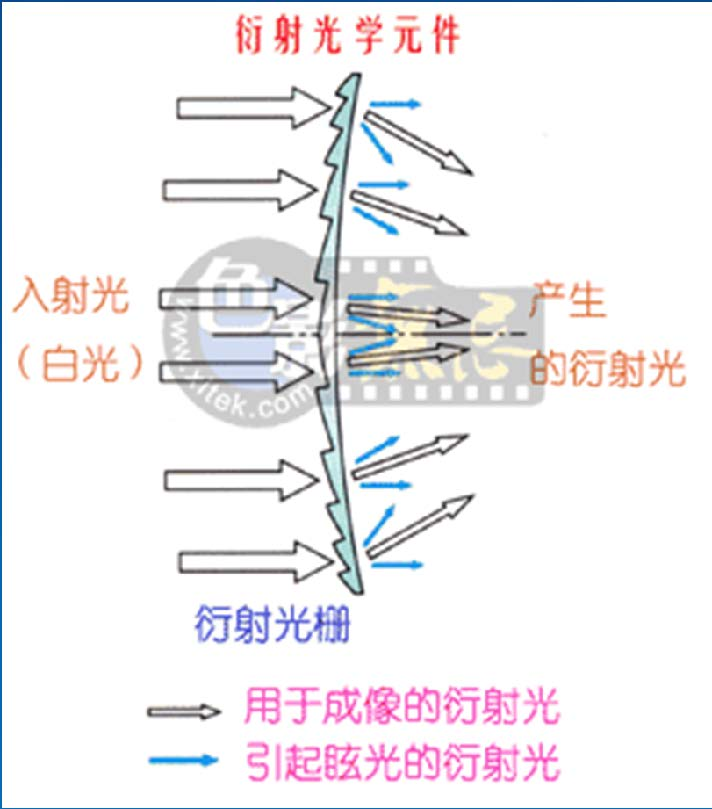
\includegraphics[height=4cm]{figure/Chapter2/衍射光学元件的衍射}}\quad
	\subfloat[DOE物镜后的区场扫描示意图]{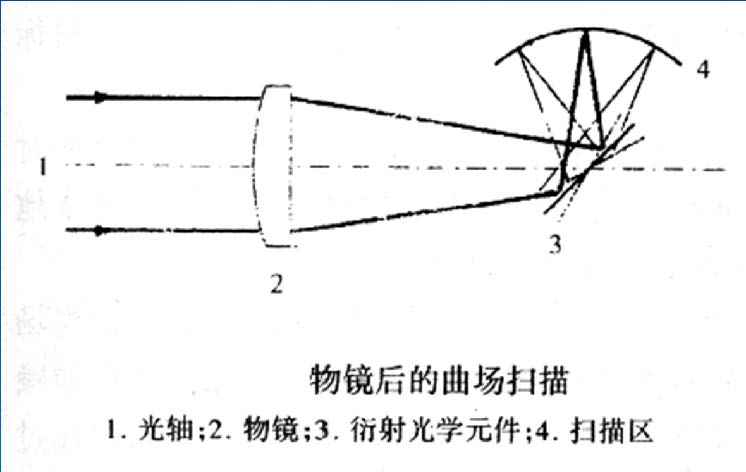
\includegraphics[height=4cm]{figure/Chapter2/DOE物镜后的区场扫描示意图}}
	\caption{衍射光学元件}
	\label{fig:衍射光学元件}
\end{figure}

\subsection{信号接收的探测技术} % Subsection 3.4	信号接收的探测技术
\paragraph{直接探测}将接收到的激光能量聚焦到光敏元件上,产生与入射光功率成正比的电压或电流。与传统的光学接收系统原理基本上相同。
\paragraph{相干探测}探测器接收目标回波信号和某一参考波的相干混合波信号,按照参考波的辐射源及其特性的不同进行探测。分为外差探测,零拍探测和多频外差探测等。
\begin{enumerate}
	\item \textit{外差探测}:
		一般外差探测激光雷达系统由一台连续工作的激光器作为独立辐射源发出参考波,称为\textit{本地振荡器}。
		系统接收到的回波信号与来自本地振荡器的参考信号混合之后,由混频器输出的光束聚焦到探测器上然后再进行信号处理。原理如图\ref{fig:外差探测}所示。
		\begin{figure}[htbp]
			\centering
			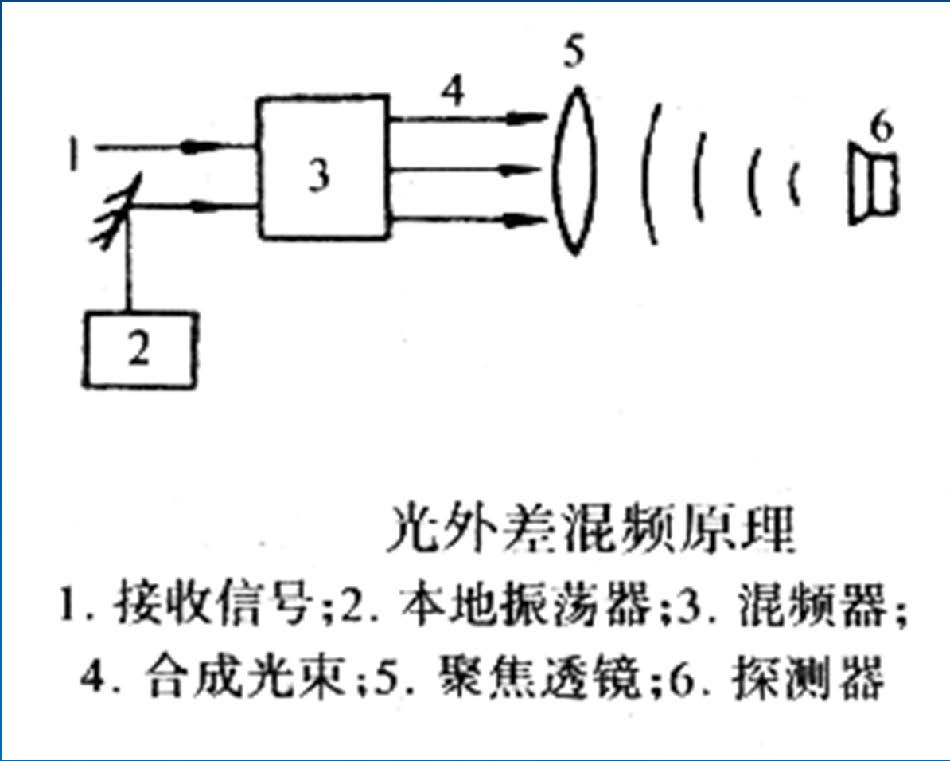
\includegraphics[width=0.5\linewidth]{figure/Chapter2/外差探测}
			\caption{外差探测原理}
			\label{fig:外差探测}
		\end{figure}
	\item \textit{零拍探测}:
		本地振荡信号是来自激光发射源的部分激光辐射,不需要另一个激光源。
		零拍激光雷达比普通外差激光雷达结构更简单,可靠性也更好。
		原理如图所示。
		\begin{figure}[htbp]
			\centering
			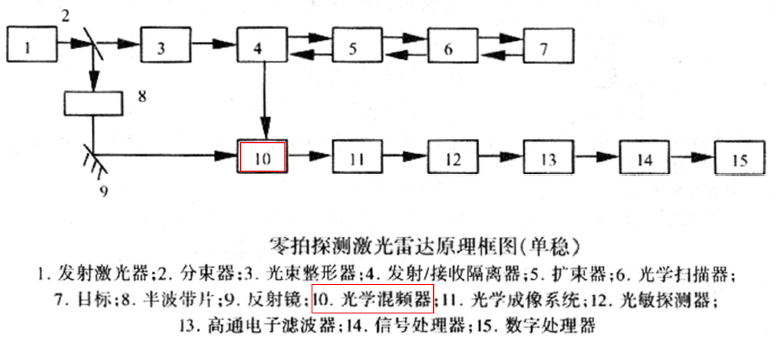
\includegraphics[width=0.7\linewidth]{figure/Chapter2/零拍探测}
			\caption{零拍探测}
			\label{fig:零拍探测}
		\end{figure}
	\item \textit{多频外差探测}:
		目标与激光雷达的相对运动产生接收信号的多普勒(Doppler)频移,可以提供有关目标的非常精确的信息;
		这要求外差探测接收器具有很宽的频带,以覆盖回波信号的频率和外差探测信号频率;
		但增加带宽会提高噪声水平,降低探测概率,解决这一问题的办法是采用三频外差系统。
		
		\textit{三频外差探测}:激光发射有两个独立辐射源,两束激光沿同一光轴向目标传播,经运动目标产生多普勒频移后返回接收器,两个反射信号与本地振荡器信号混频,成像在光敏探测器上。原理如图\ref{fig:三频外差探测系统示意图}所示。
		\begin{figure}[htbp]
			\centering
			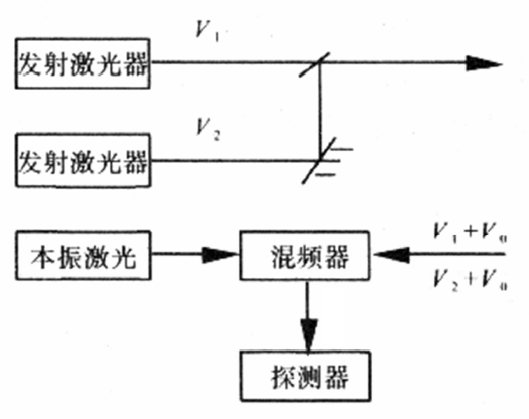
\includegraphics[width=0.5\linewidth]{figure/Chapter2/三频外差探测系统示意图}
			\caption{三频外差探测系统示意图}
			\label{fig:三频外差探测系统示意图}
		\end{figure}
\end{enumerate} % 相干探测的分类

\paragraph{接收孔直径}
\begin{itemize}
	\item 在相干探测激光雷达中,系统的有效接收孔径受散斑现象\footnote{被激光照明的物体,其表面呈现颗粒状结构。}的限制,不能任意扩大。
	\item 当接收孔径小于和等于散斑瓣的平均直径的情况下,接收功率是随接收孔的面积(孔径平方)线性增加;
	\item 在接收孔径增大,大于散斑瓣平均直径的情况下,接收功率不再服从与接收孔径面积线性相关的规律,而是与孔径线性相关;
		这种信号采集效率的下降是接收孔面积增大、反射信号相干性变差的结果;
	
		当接收孔径大于散斑瓣的平均直径时,接收孔有效直径可以表示为
		\begin{equation}
		D = \sqrt{D_rd_s}
		\end{equation}
		其中,$ D_r $表示接收器孔径实际大小,$ d_s $表示散斑瓣直径。
\end{itemize}

\section{激光信号的大气衰减}

\paragraph{激光的大气干扰}两次通过大气,不可避免受到干扰。由于激光光束波长较短,干扰主要有
\begin{itemize}
	\item 大气对它的吸收和散射作用较强,因此大气穿透能力较差。
	\item 大气中雨滴、尘埃、雾、霾等对激光的干扰作用大。
\end{itemize} % 激光的大气干扰

\paragraph{激光大气干扰的表现}
\begin{itemize}
	\item \textbf{衰减}:气体分子和气溶胶粒子、尘埃、雾、雨等的吸收和散射。
	\item \textbf{折射}:由于大气密度分布不均匀,导致激光沿光路产生折射。
	\item \textbf{其他}:大气湍流,导致光束扩展和漂移;大气吸收,引起光束相位变化。
\end{itemize} % 激光大气干扰的表现

\paragraph{激光雷达的性能}
\begin{itemize}
	\item 激光雷达的性能是与激光在大气中的传播特性密切相关的。
	\item 激光的传播特性主要与大气吸收、散射和折射的效应有关。
	\item 要充分发挥激光雷达的效能,就应充分了解激光的大气传播特性,寻找避免或克服大气效应的措施,减少大气衰减,并根据对激光在大气中的传播的规律,仔细选择激光工作波长以及激光工作方式,保证激光光束具有较高的透过率。
\end{itemize}

\subsection{大气衰减效应} % Subsection 4.1	大气衰减效应

\paragraph{布格埃—朗伯特定律}光束传播路径上大气均匀或分层均匀的情况下,目标处的光强可用布格埃—朗伯特定律描述:
\begin{equation}
I(\lambda,z) = I(\lambda,0)e^{-\sigma(\lambda)z}
\end{equation}
式中,$ z $为传播距离,$ I(\lambda,0) $、$ I(\lambda,z) $分别是波长为$ \lambda $的激光光束的初始光强和在距光源$ z $处的光强,$ \sigma(\lambda) $是与波长有关的衰减系数。

\paragraph{大气透过率}当激光束没有出现非线性效应时,大气透过率可以表示为
\begin{equation}
\tau(\lambda) = \exp\left\lbrace -\int_{0}^{L}\sigma(\lambda)\diff r \right\rbrace 
\end{equation}
其中$ L $是传播距离。对于水平平均光程,透过率可以写成
\begin{equation}
\tau(\lambda) = \exp\left\lbrace - \sigma(\lambda)L \right\rbrace
\end{equation}

\paragraph{总的衰减系数}
\begin{equation}
\sigma(\lambda) = \sigma_m + K_m + \sigma_a + k_a
\end{equation}
其中,$ \sigma_m $为分子散射系数,$ K_m $为分子吸收系数,$ \sigma_a $为气溶胶散射系数,$ k_a $为气溶胶吸收系数。
\begin{enumerate}
	\item \textbf{大气分子吸收——吸收系数}
		\begin{enumerate}
			\item \textbf{线吸收}:与单色光波长相应的大气分子的吸收。吸收系数:
				\begin{itemize}
					\item 高度在20 km以内,主要由碰撞压力展宽决定:
						\begin{equation}
						K_{ml} = \dfrac{S}{\pi}\dfrac{r_L}{(v-v_0)^2 + r_L^2}
						\end{equation}
						式中,$ v $是激光的波数,$ v_0 $是激光谱线中心的波数,$ S $为谱线的积分强度,$ r_L $为洛伦兹线半宽度,$ \alpha_D = S \cdot r_D $。
					\item 高度60 km以上,主要由多普勒展宽决定:
						\begin{equation}
						K_{MD} = \dfrac{S}{\alpha_D}\left[\dfrac{\ln 2}{\pi}\right]^{\dfrac{1}{2}} e^{-\frac{\ln 2(v-v_0)^2}{r_D^2}}
						\end{equation}
						式中,$ r_D $是多普勒谱线半宽度,$ \alpha_D = S \cdot r_D $,
						\begin{equation}
						r_d = \dfrac{v_0}{c}\left[\dfrac{2\ln 2k_BT}{M}\right]^{\frac{1}{2}} = 3.58 \times 10^{-7} \left[\dfrac{T}{M}\right] ^ {\frac{1}{2}}
						\end{equation}
					\item 在20$ \sim $60 km高度上,两种形式的吸收同时发生作用。
				\end{itemize} % 线吸收的吸收系数
			\item \textbf{连续吸收}:大气窗口内的大气分子。其吸收特点:
				\begin{itemize}
					\item 是随着光频率连续缓慢变化的分子吸收
					\item 在没有吸收线或只有很弱吸收的波长上,连续吸收成为主要因素
				\end{itemize}
				根据Kneizys得出的水汽连续吸收经验公式:
				\begin{itemize}
					\item 对10.6 μm的\ce{CO2}激光,必须考虑水汽和\ce{CO2}的连续吸收。
					\item 对10.6 μm的YAG激光,其连续吸收可以不加考虑。
				\end{itemize}
				在大气窗口内,水汽的连续吸收必须十分注意的。
		\end{enumerate} % 大气分子吸收——吸收系数
	\item \textbf{大气分子的散射}
		\begin{itemize}
			\item \textbf{瑞利散射}——大气分子。在光的波长远远大于大气中粒子之时, 大气散射表现为瑞利散射,散射系数的经验公式为
				\begin{equation}
				\sigma_m = 2.677 \times 10^{-17} \symrm{PV}^4/\symrm{T}
				\end{equation}
				其中,$ v $为波数。
			\item \textbf{米氏散射}——雨滴、雾滴、霾等粒子。当大气微粒直径很大,与激光波长可比拟之时大气散射服从米氏散射规律,一般说来,米氏散射是气溶胶散射。气溶胶粒子的总衰减系数近似表示:
				\begin{equation}
				\sigma_T = \sigma_a \sigma_m = \dfrac{3.912}{V_M} \left[\dfrac{0.55}{\gamma_{um}}\right]^b
				\end{equation}
				\begin{itemize}
					\item $ V_M $是能见度,即人眼可以辨别目标的最大距离。
					\item $ b $与能见度相关,
						\begin{itemize}
							\item 在一般条件下,$ V_M $为6$ \sim $20 km,$ b=1.3 $。
							\item 能见度特别好,$ V_M > $20 km时,$ b=1.6 $。
							\item 能见度小于6 km时,$ b = 0.585 $。 
						\end{itemize} % b
				\end{itemize} % 米氏散射
		\end{itemize} % 大气分子的散射
		总体说来, 大气分子和气溶胶的散射系数服从高度的负指数规律:随着高度的增加,散射系数很快减小。
		\begin{itemize}
			\item 在5 km以上——气溶胶散射系数与地面相比一般相差一个量级以上。
			\item 接近地面和低空中——气溶胶散射是主要的。
			\item 高空——分子散射与气溶胶散射的效果相当。
		\end{itemize}
\end{enumerate} % 衰减影响因素

\subsection{大气折射效应} % Subsection 4.2	大气折射效应

\paragraph{大气折射效应}激光通过大气时因不同的折射率造成光程增加,传播路径弯曲。

\paragraph{折射率}大气密度随着高度不同而变化,在不同的高度上大气对光的折射率不相同。大气折射率$ n $与激光波长$ \lambda $、空气的温度$ T $、湿度$ e $、压强$ P $有关
\begin{equation}
n = 1 + N(\lambda,T,P,e)
\end{equation}
式中,$ N $为\textit{折射率模数},单位为$ 10^{-6} $,一般简化写成$ N = 0.79 \times \symrm{P/T} $

\section{激光雷达系统能量方程} % Section 5 激光雷达方程

\paragraph{激光雷达方程}激光雷达能量探测的基本数学模型;
激光雷达因与目标作用的机理不同,分为不同的类型,不同类型的激光雷达要用不同的激光雷达方程加以描述。

\paragraph{激光雷达方程的一般形式}
\begin{equation}\label{equ:激光雷达方程的一般形式}
P_r = \dfrac{\eta_o \rho T_a^2 A_r}{\pi R^2} \cdot \dfrac{A_i}{A_b}P_t
\end{equation}
式中,$ P_r $是激光雷达接收到的激光功率;$ P_t $是光学系统效率;$ \rho $是目标表面反射率,$ T_a $是单程大气透过率,$ A_r $是光学系统有效接触面积,$ R $是目标与激光雷达的距离;$ A_i $是目标被照面积(截面积);$ A_b $是目标处的光斑面积。
式\eqref{equ:激光雷达方程的一般形式}\textbf{适用于发射、接收位于同一处的激光雷达的各种应用情况。}

\paragraph{单脉冲稳频激光雷达}探测器所测得的目标,距离探测器$ R $到$ R+\diff R $,辐射源产生的波长间隔为$ [\lambda,\lambda + \diff \lambda] $的微分信号功率为
\begin{equation}
\diff P(\lambda,R) = I(\lambda,R,r)p(\lambda,R,r)\diff\lambda \diff R \diff A(R,r) 
\end{equation}
探测器所接收到的总信号功率则表示为
\begin{equation}
P(\lambda,R) = \int_{0}^{R}\diff R\int_{\Delta\lambda}\int I(\lambda,R,r)p(\lambda,R,r)\diff A(R,r)
\end{equation}
其中,$ p(\lambda,R,r) $取决于
\begin{itemize}
	\item 大气传输因子;
	\item 接收系统传输因子$ T_r(\lambda) $;
	\item 接收立体角$ \dfrac{A_0}{R^2} $;
	\item 接收视场与激光辐射照射面的重叠因子及在距离$ R $到$ R+\diff R $内回波到达探测器的概率$ p(R) $。
\end{itemize} % p(\lambda,R,r)取决于
